\message{ !name(lect08.ltx)}
\message{ !name(lect08.ltx) !offset(-2) }
\documentclass[landscape]{slides}

\usepackage{amsmath,amssymb}
\usepackage[pdftex]{graphicx}

\newcommand{\lecnum}{AGM-08}
\newcommand{\slidehead}[1]{{\centering \bf #1 \\}}
\newenvironment{titledslide}[1]{\begin{slide}\slidehead{#1}\vfill}{\vfill \tiny \lecnum \end{slide}}

\newcommand{\variables}{\ensuremath{\Delta}}
\newcommand{\variable}{\ensuremath{\delta}}
\newcommand{\cell}{\ensuremath{i}}
\newcommand{\table}{\ensuremath{{\cal I}}}
\newcommand{\values}{\ensuremath{{\cal I}_\delta}}
\newcommand{\reals}{\ensuremath{{\cal R}}}
\newcommand{\hg}{\ensuremath{{\cal H}}}
\newcommand{\gr}{\ensuremath{{\cal G}}}
\newcommand{\ci}[3]{\ensuremath{#1 \perp #2 | #3}}

\begin{document}

%%%%%%%%%%%%%%%%%%%%%%%%%%%%%%%%%%%%%%%%%%%%%%%%%%%%%%%%%%%%%%%%%%%%%%
\begin{titledslide}{Algorithms for Graphical Models (AGM)\\
\vfill {\Huge Bayesian nets}}\vfill

\begin{verbatim}
$Date: 2006/09/07 14:54:53 $
\end{verbatim}

\end{titledslide}
%%%%%%%%%%%%%%%%%%%%%%%%%%%%%%%%%%%%%%%%%%%%%%%%%%%%%%%%%%%%%%%%%%%%%%
\begin{titledslide}{In this lecture}

  Bayesian nets:
    \begin{itemize}
    \item what they are
    \item conditional independence properties
    \item as factored distributions
    \end{itemize}



\end{titledslide}  
%%%%%%%%%%%%%%%%%%%%%%%%%%%%%%%%%%%%%%%%%%%%%%%%%%%%%%%%%%%%%%%%%%%%%%
\begin{titledslide}{Bayesian net structure}
  
  \begin{itemize}
  \item The structure of a Bayesian net is given by a directed acyclic
    graph (DAG) whose nodes are the variables of a distribution.
  \item Here's one for the `Asia' example:
  \end{itemize}

  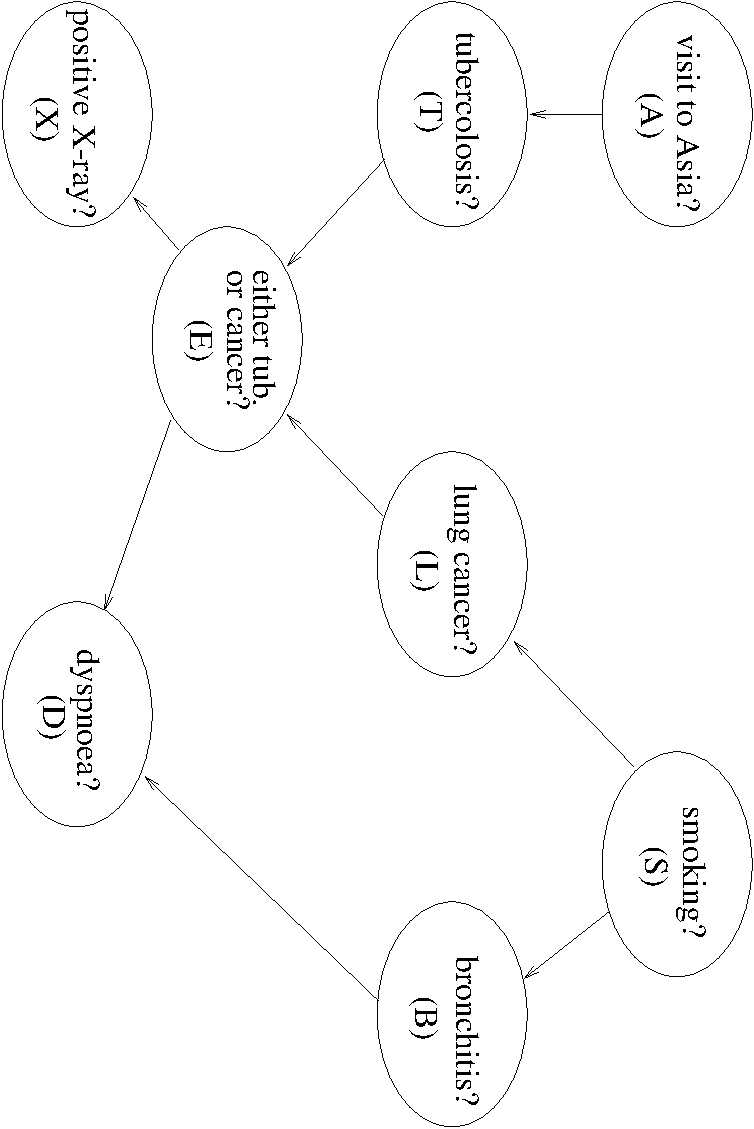
\includegraphics[width=6cm,height=20cm,angle=90]{asia.pdf}

\end{titledslide}
%%%%%%%%%%%%%%%%%%%%%%%%%%%%%%%%%%%%%%%%%%%%%%%%%%%%%%%%%%%%%%%%%%%%%%
\begin{titledslide}{Directed graph terminology}
  
  \begin{itemize}
  \item If there's an arrow $A \rightarrow B$ is a directed graph,
    then $A$ is a \emph{parent} of $B$ and $B$ is a \emph{child} of $A$.
  \item A directed graph (digraph) is \emph{acyclic} if the graph
    contains no loops which follow the direction of the arrows.
  \item The DAG defines a partial order on nodes. A (total) ordering
    of nodes consistent with a given DAG is one consistent with this
    partial ordering.
  \end{itemize}

\end{titledslide}
%%%%%%%%%%%%%%%%%%%%%%%%%%%%%%%%%%%%%%%%%%%%%%%%%%%%%%%%%%%%%%%%%%%%%
\begin{titledslide}{Bayesian net parameters}
  
  \begin{itemize}
  \item There is a \emph{conditional probability table (CPT)} for each
    variable.
  \item The CPT for variable $X$ defines a distribution over the
    values of $X$ \emph{for each joint instantiation of the parents of
      $X$}
  \item Here are the CPTs for Asia. Cue \verb+asia_cpts.py+
  \end{itemize}


\end{titledslide}
%%%%%%%%%%%%%%%%%%%%%%%%%%%%%%%%%%%%%%%%%%%%%%%%%%%%%%%%%%%%%%%%%%%%%%
\begin{titledslide}{The distribution represented by a Bayesian net}

  \begin{itemize}
  \item Note that each CPT is a factor.
  \item The distribution represented by a Bayesian net is the product
    of all the CPTs.
  \item So BNs are factored distributions and so everything we have
    said about more general factored distributions holds for BNs as well.
  \item But (unsurprisingly!) BNs have extra properties.
  \end{itemize}
  
\end{titledslide}
%%%%%%%%%%%%%%%%%%%%%%%%%%%%%%%%%%%%%%%%%%%%%%%%%%%%%%%%%%%%%%%%%%%%%%
\begin{titledslide}{No normalisation needed}
  
  \begin{itemize}
  \item A product of CPTs, one for each variable, defines a
    distribution directly, no matter what numbers are in the CPTs \dots
  \item \dots \emph{as long as the corresponding digraph is acyclic}.
  \item There is no need to normalise: you will prove this as an
    exercise.
  \end{itemize}

\end{titledslide}
%%%%%%%%%%%%%%%%%%%%%%%%%%%%%%%%%%%%%%%%%%%%%%%%%%%%%%%%%%%%%%%%%%%%%%
\begin{titledslide}{The moral graph}
  
  \begin{itemize}
  \item If we `forget' that the CPTs are CPTs and just treat them as
    factors, then the resulting interaction graph is called the
    \emph{moral graph}.
  \item Unmarried parents get connected (since they are together in
    some CPT) and the arrows disappear (since the CPTs loose their CPTness).
  \item It's not difficult to see that a BN \emph{factorises according
    to its moral graph}.
  \end{itemize}

\end{titledslide}
%%%%%%%%%%%%%%%%%%%%%%%%%%%%%%%%%%%%%%%%%%%%%%%%%%%%%%%%%%%%%%%%%%%%%%
\begin{titledslide}{Conditional independencies from a BN's moral graph}
  
  \begin{itemize}
  \item Since a BN factorises according to its moral graph, we can
    read off some conditional independencies from its moral graph.
  \item For example, we have that $\ci{\{A\}}{\{B,D,S\}}{\{E,L,T\}}$.
  \item However, there are further conditional independence relations
    which hold in a BN but cannot be deduced from the moral graph.
  \item To get these we need to exploit properties of CPTs \dots
  \end{itemize}

\end{titledslide}
%%%%%%%%%%%%%%%%%%%%%%%%%%%%%%%%%%%%%%%%%%%%%%%%%%%%%%%%%%%%%%%%%%%%%%
\begin{titledslide}{The key property of CPTs}
  
  \begin{itemize}
  \item For any configuration of its parents the values for
    the child must add up to one: this is what makes it a CPT.
  \item So if we marginalise away the child variable in a CPT we end
    up with a factor of ones.
  \item Factors with all data values = 1 can be deleted from a
    factored distribution without altering the distribution.
  \item So if a variable only appears in its own CPT then we can
    marginalise it away from the Bayesian net by simply removing this CPT!
  \end{itemize}

\end{titledslide}
%%%%%%%%%%%%%%%%%%%%%%%%%%%%%%%%%%%%%%%%%%%%%%%%%%%%%%%%%%%%%%%%%%%%%%
\begin{titledslide}{Removing childless variables from Bayesian nets}
  
  \begin{itemize}
  \item Let $P(A,T,E,L,S,B,D,X)$ be the joint distribution defined by
    the `Asia' Bayesian net.
  \item The marginal distribution $P(A,T,E,L,S,B,X)$ [$D$ marginalised
    away] is given by the BN with (i) the CPT for $D$ deleted and thus
    (ii) the node $D$ and all links to it deleted in the corresponding
    acyclic digraph. 
  \item The BN for $P(A,T,E,L,S,X)$ [$B$ marginalised away in
    addition] is produced by deleting $B$ from the BN for $P(A,T,E,L,S,B,X)$.
  \item Clearly there is some sort of general principle here \dots
  \end{itemize}

\end{titledslide}
%%%%%%%%%%%%%%%%%%%%%%%%%%%%%%%%%%%%%%%%%%%%%%%%%%%%%%%%%%%%%%%%%%%%%%
\begin{titledslide}{Ancestral sets}
  
  \begin{itemize}
  \item In a given digraph, the \emph{ancestors} of vertex $X$,
    denoted $an(X)$, is the set of nodes $Y$ such that there is a
    directed path from $Y$ to $X$.
  \item It's just the transitive closure of the parent relationship.
  \item A set of nodes $\mathbf{X}$ is an \emph{ancestral set} iff for
    any node $X \in \mathbf{X}$ we have $an(X) \subseteq \mathbf{X}$.
  \item Let $An(\mathbf{Z})$ denote the smallest ancestral set
    containing a set of nodes $
  \end{itemize}

\end{titledslide}
%%%%%%%%%%%%%%%%%%%%%%%%%%%%%%%%%%%%%%%%%%%%%%%%%%%%%%%%%%%%%%%%%%%%%%
\begin{titledslide}{Ancestral sets by example}
  
  \begin{itemize}
  \item Some ancestral sets in the `Asia' digraph:\\ $\emptyset,
    \{B,L,S\}, \{A,E,L,S,T\}, \{A,B,E,L,S,T\}, \{A,S\}$.
  \item And some sets which are not ancestral:\\ $\{L\}, \{A,E,L,S\}$.
  \end{itemize}

\end{titledslide}
%%%%%%%%%%%%%%%%%%%%%%%%%%%%%%%%%%%%%%%%%%%%%%%%%%%%%%%%%%%%%%%%%%%%%%
\begin{titledslide}{The key property of Bayesian nets}
  
  \begin{itemize}
  \item (Notation: Let $P$ be a joint distribution and $\mathbf{X}$ be
    some subset of its variables, then denote the distribution
    produced by marginalising $P$ onto $\mathbf{X}$ as
    $P_{\mathbf{X}}$. If \gr{} is a graph, let $\gr_{\mathbf{X}}$ be the
    graph formed by removing from \gr{} all nodes not in $\mathbf{X}$.)
  \item Let $P$ be defined by a BN with acyclic digraph \gr{} and let
    $\mathbf{X}$ be an ancestral set in \gr \dots
  \item \dots then $P_{\mathbf{X}}$ is given by the BN with DAG
    $\gr_{\mathbf{X}}$ (and the relevant CPTs deleted).
  \end{itemize}

\end{titledslide}
%%%%%%%%%%%%%%%%%%%%%%%%%%%%%%%%%%%%%%%%%%%%%%%%%%%%%%%%%%%%%%%%%%%%%%
\begin{titledslide}{What this means for conditional independence}

  \begin{itemize}
  \item If we want to know whether the BN structure implies
    $\ci{\mathbf{A}}{\mathbf{B}}{\mathbf{S}}$ for disjoint sets of
    variables $\mathbf{A}, \mathbf{B}, \mathbf{S}$
  \end{itemize}
  
\end{titledslide}
%%%%%%%%%%%%%%%%%%%%%%%%%%%%%%%%%%%%%%%%%%%%%%%%%%%%%%%%%%%%%%%%%%%%%%
\begin{titledslide}{Conditional independence in BNs}
  
  By definition our `Asia' BN defines a joint distribution as follows:
  \begin{multline*}
    P(A,T,E,L,S,B,D,X) = \\
    P(X|E)P(D|E,B) 
    P(E|T,L)P(B|S)\\
    P(L|S)P(S)P(T|A)P(A)
  \end{multline*}

But for \emph{any} distribution we also have:

\begin{multline*}
  P(A,T,E,L,S,B,D,X) = \\
  P(X|A,T,E,L,S,B,D)P(D|A,T,E,L,S,B) \\
  P(E|A,T,L,S,B)P(B|A,T,L,S)\\
    P(L|A,T,S)P(S|A,T)P(T|A)P(A)\\
  \end{multline*}

\end{titledslide}
%%%%%%%%%%%%%%%%%%%%%%%%%%%%%%%%%%%%%%%%%%%%%%%%%%%%%%%%%%%%%%%%%%%%%%


%%%%%%%%%%%%%%%%%%%%%%%%%%%%%%%%%%%%%%%%%%%%%%%%%%%%%%%%%%%%%%%%%%%%%%

\end{document}

\message{ !name(lect08.ltx) !offset(-248) }
